
\chapter{Abordagem \textit{GAHME}}\label{chapter:abordagem_gahme}
A abordagem \textit{GAHME} é um modelo de monitoramento de dados motores de saúde por meio de jogos eletrônicos. Para essa abordagem tornar-se viável, é necessário primeiramente realizar um estudo sobre quais os movimentos e ações o usuário deve exercer para que os sinais motores sejam capturados corretamente e torne possível a identificação dos sintomas. De posse dos movimentos, estes devem ser testados junto a indivíduos portadores da deficiência a ser monitorada e indivíduos como grupo de controle para avaliar a detecção do sintoma.


\section{Definição de Requisitos da Solução}\label{section:requisitos_solucao}
Com base no levantamento bibliográfico e em entrevistas preliminares com profissionais de saúde, os seguintes requisitos funcionais foram definidos para a solução \textit{GAHME}:

\begin{description}
	\item[REQ-GAHME-01 - Pontuação e Taxa de Acerto]: O jogador percebe os objetivos e visualiza o sucesso ou fracasso alcançado. O jogo pontua o jogadora de acordo com seus seus erros e acertos~\cite{Suhonen:2008:SFE:1457199.1457204,sinclair07}.
	\item[REQ-GAHME-02 - Progresso e Evolução do Jogador e dos Desafios]: O jogador percebe seu progresso e evolução no jogo. Os desafios tonam-se mais complexos no decorrer do tempo ~\cite{Suhonen:2008:SFE:1457199.1457204}.
	\item[REQ-GAHME-03 - Estado de Fluxo]: Um dos grandes desafios de um jogo eletrônico é levar o usuário a um ``Estado de Fluxo'' ou escapismo passando a executar a atividade proposta pelo jogo de uma forma autotélica, ou seja o usuário não vislumbra um benefício imediato ou futuro ~\cite{sweetser2005-gameflow}. 
	\item[REQ-GAHME-04 - Preocupação com Integridade Física do Jogador]: Promover atividades físicas, ou ações que venham a trazer injúria ao jogador, como movimentos de equilíbrio, movimentos repetitivos ou bruscos ~\cite{sinclair07,arntzen2011}.
		\item[REQ-GAHME-05 - Captura e Armazenamento de Sinais Motores]: O jogo deve realizar a captura dos sinais motores do usuário usando sensores de movimento. Os dados capturados são enviados à um servidor para tornar possível o acompanhamento da saúde motora.
	\item[REQ-GAHME-06 - Mecanismo de Identificação de Sintomas Motores]: Baseados em algoritmos de aprendizagem de máquina o servidor acompanha todos os usuários do sistema e identifica qual deles está com distúrbio motor, em caso afirmativo envia-se a informação ao profissional de saúde.
	\item[REQ-GAHME-07 - Mecanismo de Visualização dos Parâmetros Motores do Usuário]: O profissional de saúde poderá visualizar os dados identificados pela máquina de aprendizagem para realizar a tomada de decisão sobre o estado de saúde do usuário.
\end{description}

\section{Visão geral da solução}

A abordagem \textit{GAHME} faz uso de jogos eletrônicos como interface de captura, tornando os usuários mais motivados a fornecer os dados motores, em comparação ao uso dos dispositivos vestíveis. Desta forma, o profissional de saúde poderá visualizar os dados motores capturados em um momento em que o usuário está descontraído sem a preocupação de estar participando de um exame motor. 

\begin{figure}[!htb]
     \centering
     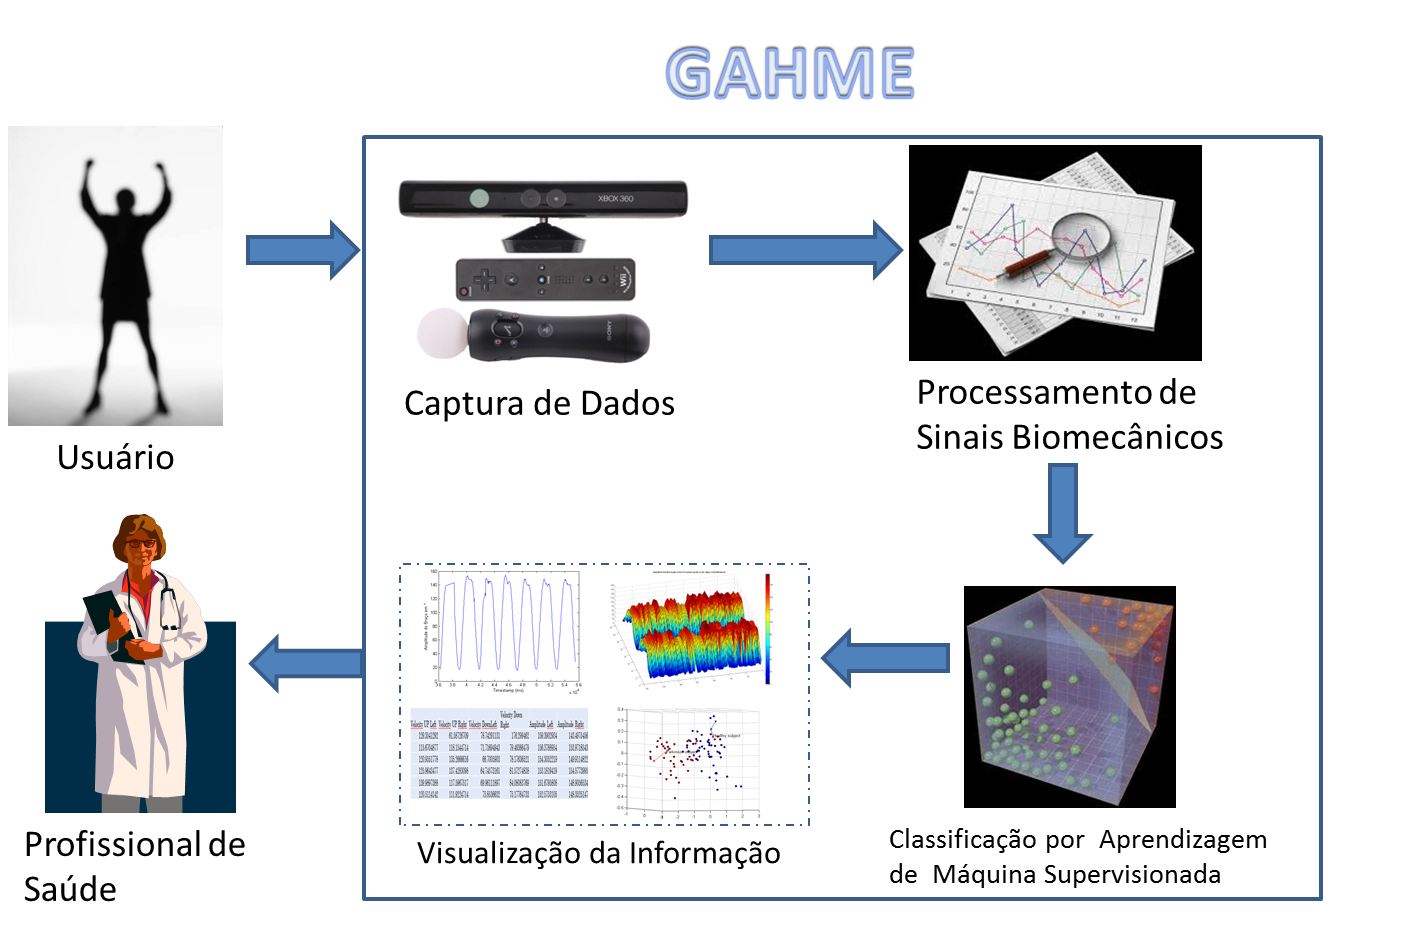
\includegraphics[width=1\textwidth]{./img/systemoverview.png}
     \caption{Visão Geral da Abordagem \textit{GAHME}}
     \label{img:visaogeral}
\end{figure}

Com o uso dos jogos eletrônicos é possível alcançar requisitos de pervasividade e não invasividade. Pois através dos dispositivos de sensores de movimento usados nesses ambientes, é possível desenvolver um jogo que motive o usuário a executar ações específicas que permitam o monitoramento de dados motores. A partir de uma interface com o usuário que permite enviar os dados capturados a um servidor, este fará o armazenamento dos dados para um possível acompanhamento da saúde motora.

Baseado em técnicas de processamento de sinais e reconhecimento de padrões, será possível identificar sintomas motores. Esta abordagem consiste em realizar o processamento dos dados com o objetivo de filtrar ciclos de movimento que permitam identificar sinais motores e como consequência seja possível extrair as características desse movimento. Após a extração das características, os dados são repassados para Máquinas de Aprendizagem que classificam os dados por meio das evidências estatísticas. Caso a máquina identifique algum usuário com distúrbio motor, ela poderá notificar o Profissional de Saúde e este poderá visualizar os dados para uma melhor tomada de decisão, como pode ilustrado na Figura~\ref{img:visaogeral}.

%A abordagem \textit{GAHME} pode ser vista como uma caixa preta que recebe como entrada os dados motores de indivíduos e tem como saída técnicas de aprendizagem de máquina para identificar a ocorrência sintomas motores. Caso a máquina de aprendizagem identifique algum problema motor em um indivíduo o Profissional de saúde poderá visualizar os dados e realizar a tomada de decisão sobre o tratamento.

%O Processamento de Sinais Biomecânicos e a Aprendizagem Supervisionada usam classificadores de dados. Esses módulos realizam o processamento dos dados com o objetivo de filtrar ciclos de movimento que possibilitem a identificação de sinais de motores de saúde e como consequência possam extrair as características desse movimento. Após a extração das características, os dados são repassados para Máquinas de Aprendizagem que classificam os dados por intermédio das evidências estatísticas encontradas neles como iremos explicar no decorrer deste capítulo.

O funcionamento da abordagem pode ser descrito como uma composição de quatro passos: captura dos sinais através de sensores, processamento de sinais biomecânicos, classificação dos dados e visualização.

\section{Aquisição de Dados}
O propósito de um \textit{GAHME} é coletar informações do estado motor dos indivíduos de forma não invasiva. Por este motivo, foi apresentada uma abordagem de jogos eletrônicos como infraestrutura de captura de dados motores por meio dos sensores de movimento utilizados.

O cliente \textit{GAHME} é um jogo com funcionalidades de aquisição de dados motores de movimentos específicos. Logo, ele realiza a captura e envio de dados para um servidor que recebe requisições para efetuar o recebimento e armazenamento das informações. Tornando possível armazenar o histórico do usuário para um acompanhamento dos sinais motores por um longo período. Desta maneira um profissional de saúde poderá visualizar a evolução da saúde motora do usuário.

\section{Processamento de Dados Biomecânicos}\label{sec:processador_bio}
O módulo de Processamento de Dados Biomecânicos é responsável por: filtrar, remover ruídos e identificar ciclos de movimento para uma posterior extração dos vetores de características. A partir dos dados processados, aplicam-se técnicas de aprendizagem de máquina para obter a classificação dos dados e consequentemente testar as hipóteses apresentadas nesta proposta.

\subsection{Identificação de Ciclos de Movimento}\label{section:identificao_ciclos}

Os sinais adquiridos por sensores de movimento possuem bastante ruído, o que dificulta na identificação dos ciclos de movimento, pois eles possuem uma posição que inicia o ciclo de movimento como na Figura~\ref{img:exsinalposicaopunho} e o ruído existente pode cruzar por essa linha e consequentemente gerar falsas identificações. Métodos que fazem uso de filtros de passa baixa podem ser aplicados para suavizar a curva e diminuir a ocorrência do ruído, contudo isso implica numa alteração no tempo do sinal o que impacta diretamente no cálculo das características do movimento e como consequência na acurácia do resultado final ~\cite{peakdetect}.

\begin{figure}[!htb]
     \centering
     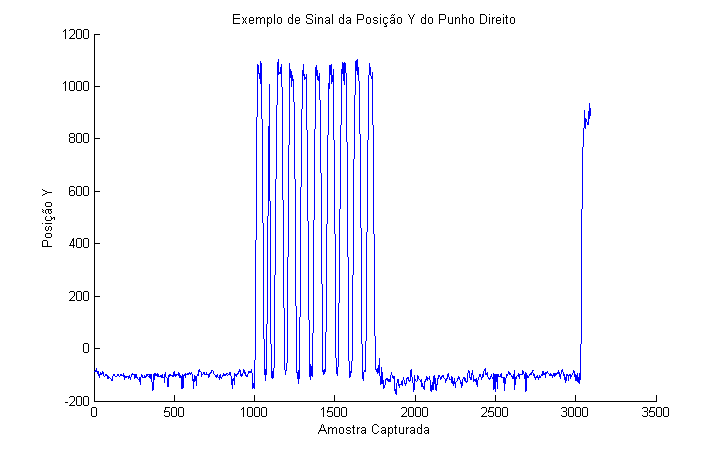
\includegraphics[width=1\textwidth]{./img/exsinalposicaoypunhodireito.png}
     \caption{Exemplo de Sinal Capturado da Articulação do Punho do Direito Usando MS-Kinnect na Posição Y}
     \label{img:exsinalposicaopunho}
\end{figure}

Em casos de análise de dados biomecânicos da amplitude do movimento é possível aplicar a técnica de detecção de picos e vales do sinal. Esta técnica consiste em usar um valor de referência $\delta$\ (\textit{delta}) para identificação dos picos e descartar valores menores que são considerados ruídos. O pico é o ponto mais alto entre os 2 pontos mais baixos que são considerados os vales do ciclo~\cite{peakdetect}. A técnica é aplicada no sinal da Figura~\ref{img:exsinalposicaopunho} com um $\delta$\ de 500 e teve como resultado os picos e os vales identificados como pode ser visto na Figura~\ref{img:expicosvales}.

\begin{figure}[!htb]
     \centering
     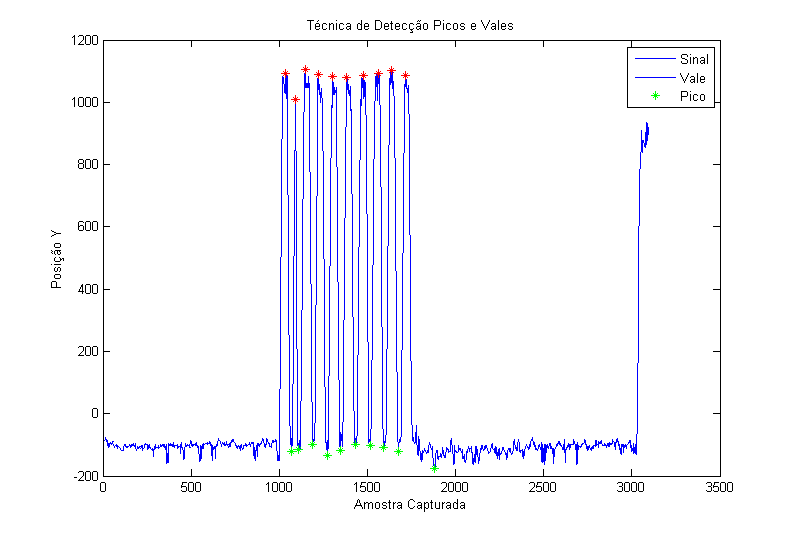
\includegraphics[width=1\textwidth]{./img/deteccaopicosvales.png}
     \caption{Exemplo da Aplicação da Técnica de Detecção de Picos e Vales no Sinal}
     \label{img:expicosvales}
\end{figure}


%\subsubsection{Redução de Ruídos no Sinal}
O processo de Identificação de Ciclos de Movimento é realizado em 3 etapas distintas:
\begin{itemize}
	\item Identificar ciclos de movimentos;
	\item calcular movimento angular realizado durante o ciclo de movimento;
	\item remover ciclos de movimentos incompletos.
\end{itemize}

Para identificar os ciclos de movimento de adução e abdução dos braços é necessário utilizar uma das articulações como referência. Neste movimento a articulação do punho (Figura~\ref{img:remocaoruidossinal}) é a que possui o sinal como maior amplitude entre as demais, por esse motivo esta é a escolhida para identificar os ciclos. Realiza-se a técnica de picos e vales no sinal do pinho para identificar o início e o fim do movimento de adução e abdução dos braços. Depois de identificado, onde começa e termina o movimento calcula-se o movimento angular através do produto escalar entre as articulações do punho, ombro e bacia(Seção~\ref{section:movimento_abducao}). Neste momento, o sinal irá conter ciclos de movimentos angulares, onde realiza-se uma nova eliminação de ruídos, ao extrair os ciclos de movimento identificados no sinal. Essa é a primeira etapa da filtragem dos dados, a qual seleciona o início e o fim dos ciclos de movimento. Depois desta etapa, realiza-se a extração de cada ciclo e identifica sua completude para que as características extraídas dos ciclos de movimento sejam semelhantes para cada indivíduo e torne possível a classificação dos dados.

\begin{figure}[!htb]
     \centering
     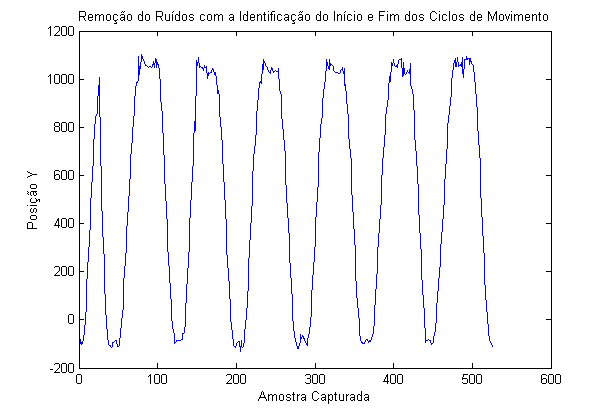
\includegraphics[width=1\textwidth]{./img/remocaoruidociclo.png}
     \caption{Remoção de Ruídos}
     \label{img:remocaoruidossinal}
\end{figure}


\subsection{Extração das Características do Movimento} \label{sec:extracao_caracteristcas}
As características do sinal a ser obtido é baseada na cinemática do movimento angular. Logo, é necessário um estudo da biomecânica do movimento humano nos ciclos de movimento ~\cite{hamill1999bases}. De posse do tempo de ocorrência de cada ciclo (\textit{Timestamp}) e das articulações do \textbf{punho}, \textbf{bacia} e \textbf{ombro} deve-se calcular o ângulo relativo do movimento de abdução e adução do braço através da aplicação do teorema do produto escalar (Equação~\ref{eq:produto_escalar}) que encontra o ângulo entre dois vetores dentro do intervalo de $0 \leq \theta \leq 180º$.

\subsubsection{Cálculo do Ângulo Relativo do Movimento de Abdução e Adução}\label{section:movimento_abducao}
O produto escalar é uma operação entre dois vetores cujo resultado é um escalar ~\cite{algebra90}. Então, o ângulo entre dois vetores é definido como ``o menor'' ângulo entre eles. Desta forma, este ângulo está dentro do intervalo de $0 \leq \theta \leq 180º $. O produto escalar é o ângulo de $ \theta$ formado entre os vetores $ v $ e $ w $ (Figura~\ref{img:produto_escalar}).


\begin{equation}
cos(\theta) = (v . w) /  (||v|| ||w||) 
\label{eq:produto_escalar}
\end{equation}


\begin{figure}[!htb]
     \centering
     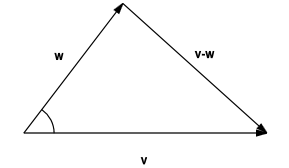
\includegraphics[width=0.5\textwidth]{./img/produtoescalar.png}
     \caption{Produto Escalar Entre 2 Vetores}
     \label{img:produto_escalar}
\end{figure}

No movimento de abdução e adução do braço (Figura \ref{fig:movabducaoaducao}), o ângulo relativo pode ser calculado com as Posições ($ x $\ ,  $ y $\ , $ z $\ ) das articulações (\textit{bacia}, \textit{ombro} e \textit{punho}). O código fonte em \textit{Matlab} ~\cite{matlab2011} realiza o cálculo do Produto Escalar dessas articulações e converte o valor escalar em °, para podermos extrair as características do movimento nessa unidade.

%O ângulo relativo podem ser calculados usando a Lei dos Cossenos. Essa lei é simplesmente um caso mais geral do Teorema de Pitágoras e descreve a relação entre os lados de um triângulo. Para nossos propósitos, o triângulo é constituído por dois segmentos (b e c) e uma linha (a) unindo a ponta distai de um segmento com a ponta proximal do outro ~\cite{hamill1999bases}.

\begin{figure}[!htb]
     \centering
     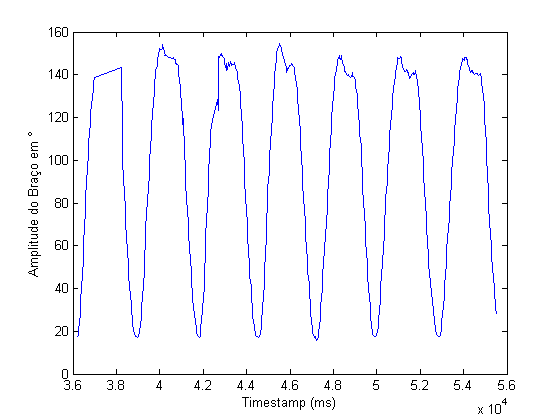
\includegraphics[width=1\textwidth]{./img/amplitude-braco.png}
     \caption{Amplitude do Movimento de Abdução e Adução}
     \label{img:amplitude_braco}
\end{figure}

Com o cálculo do produto escalar (Código Fonte~\ref{code:produto_escalar}) usando as três articulações, quantifica-se em °/ms o movimento de adução e abdução do braço em relação ao tempo criando o sinal desse movimento como na Figura~\ref{img:amplitude_braco}.

\lstset{language=Matlab}          % Set your language (you can change the language for each code-block optionally)
\begin{lstlisting}[frame=single, caption=Código do Ângulo Relativo por Produto Escalar, label=code:produto_escalar]  % Start your code-block
Bacia = [articulacaoBacia(PosicaoX), articulacaoBacia(PosicaoY), articulacaoBacia(Posicaoz)];
Ombro = [articulacaoOmbro(PosicaoX), articulacaoOmbro(PosicaoY), articulacaoOmbro(Posicaoz)];
Punho = [articulacaoPunho(PosicaoX), articulacaoPunho(PosicaoY), articulacaoPunho(Posicaoz)];

w = Bacia-Ombro;
v = Punho-Ombro;

CosTheta = dot(w,v)/(norm(w)*norm(v));
ThetaEmGraus = acos(CosTheta)*180/pi;
\end{lstlisting}

\subsubsection{Cálculo da Velocidade Angular do Movimento de Abdução e Adução}
O pico da amplitude do movimento irá conter a amplitude máxima desse movimento. O tempo gasto entre 1° vale até o pico em cada ciclo de movimento será o tempo gasto para a abdução do braço e o tempo gasto entre o pico e o 2° vale de cada ciclo será o tempo gasto para a adução do braço. Logo, com a amplitude máxima e o tempo gasto nesses movimentos podem ser calculadas as velocidades angulares de abdução e adução dos braços como na Figura~\ref{img:amplitude_braco_picos_vales}.
\begin{figure}[!htb]
     \centering
     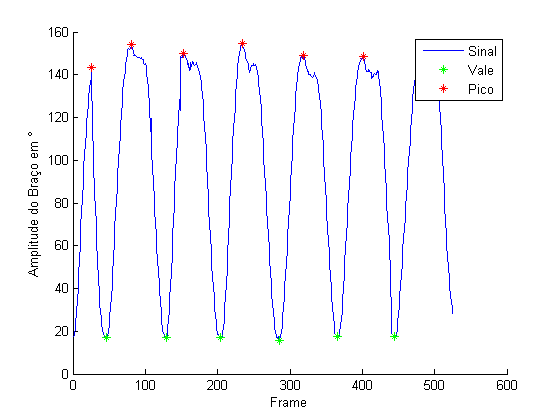
\includegraphics[width=1\textwidth]{./img/amplitude-braco-picos.png}
     \caption{Detecção de Picos e Vales da Amplitude do Movimento de Abdução e Adução do Braço}
     \label{img:amplitude_braco_picos_vales}
\end{figure}

\subsection{Filtragem de Dados}\label{section:filtro_dados}

A filtragem dos dados consiste na realização das seguintes etapas nos ciclos de movimento:
\begin{description}
	\item [Escalonar os ciclos]: O conjunto de dados deve possuir a distribuição de \textbf{M} amostras de vetores de dimensão \textbf{n}. Como os dados a serem analisados são sinais, deve-se então escalonar o sinal para uma dimensão \textbf{n} para poder realizar o cálculo matricial quadrático de (\textbf{M} x \textbf{n}).		
	\item [Normalizar os ciclos]: Em estatística o termo normalização possui diferentes significados ~\cite{statisticterms2006}. Neste trabalho, a normalização consiste no ajuste dos valores dos dados em torno do valor máximo. Ou seja o máximo valor obtido dos dados terá o valor 1 e os demais será o resultado pela divisão do valor máximo. A normalização se faz necessária para que a variação dos dados seja mantida além de facilitar a identificação de similaridades ~\cite{vicini2005}. 	
	\item [Calcular Vetor Médio dos Ciclos]: Para definir a completude de um ciclo de movimento deve-se inicialmente calcular a média entre todos os ciclos de movimento que é o vetor médio dos ciclos escalonados e normalizados (Figura ~\ref{img:ciclos_normalizado_escalonado}). O \textbf{vetor médio}, Equação (\ref{eq:vetormedio}), chamado de $\bar{X}$\ consiste na média aritmética de todos os ciclos de movimento ou seja calcula a centralização dos dados ~\cite{statisticshandbook2009}. 	
		\begin{equation}
			\bar{X}=\frac{\sum_{i=1}^{n}(Xi)}{(n)}
			\label{eq:vetormedio}
		\end{equation}
	\item [Calcular Variância de Cada Ciclo ao Vetor Médio]: A variância é uma medida de dispersão estatística, que indica o quão longe os estão de um valor esperado~\cite{statisticshandbook2009}. Neste caso o  valor esperado é o vetor médio dos ciclos ($\bar{X}$) e a variância, Equação (~\ref{eq:variancia}), irá nos informar o quão distante cada ciclo ($C$) está em relação a média.
		\begin{equation}
			var(C) = (C - \bar{X} )^2
			\label{eq:variancia}
		\end{equation}
		
		
	\item [Definir limiar para remoção de ciclos]: Essa etapa do processo de filtragem não é trivial, pois deve-se definir uma constante $ filtro $\ que será comparada à variância do ciclo, se esta for menor será aceita, caso contrário removida. Contudo,	balancear entre o limiar de dispersão do ciclo de movimento em relação a média é complexo, pois existe uma grande variabilidade de movimento. Logo, um limiar muito alto pode acarretar na remoção de uma grande quantidade de ciclos. Por outro lado, um limiar baixo pode colocar na base ciclos com ruídos e consequentemente impactar na classificação dos dados.	
	\lstset{language=Matlab}
	\begin{lstlisting}[frame=single, caption=Filtro dos Ciclos]  % Start your code-block
		
    filtro = 1;
    vetorMedio = mean(ciclos);
    varianciaCiclo = sum(ciclo - (vetorMedio).^2);
    remocao = varianciaCiclo>filtro;
	\end{lstlisting}
	
	\begin{figure}
     \centering
     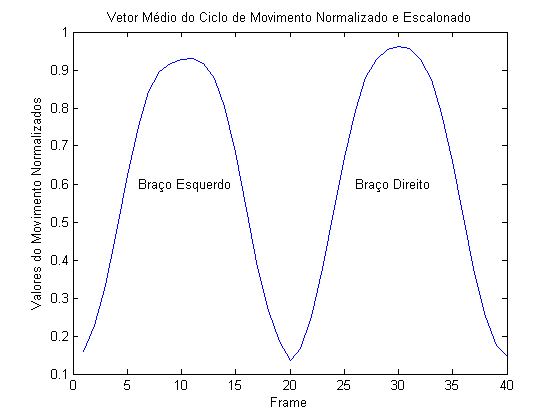
\includegraphics[width=1\textwidth]{./img/vetormedionormalozadoescalonado.png}
     \caption{Ciclos de Movimento Normalizados e Escalonados}
		 \label{img:ciclos_normalizado_escalonado}
	\end{figure}
\end{description}


%\lstset{language=Matlab}
%\begin{lstlisting}
	%normalizarCiclos(ciclos);
	%escalonarCiclos(ciclos, CONSTANTE_ESCALONAMENTO);
	%vetormedio = mean(ciclos);
	%
	%
%\end{lstlisting}

%%Média

Como exemplo, temos um ciclo de movimento filtrado (Figura~\ref{img:ciclo_filtrado}) (\textit{valor do filtro = 1}) e o (\textit{valor da variância = 2,3078}).

\begin{figure}[!htb]
     \centering
     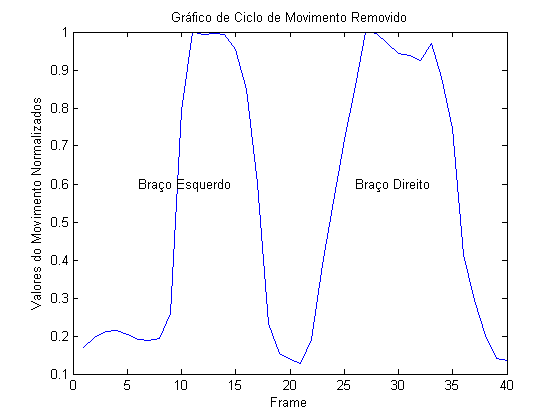
\includegraphics[width=1\textwidth]{./img/ciclomovimentoremovido.png}
     \caption{Ciclo de Movimento Removido}
		 \label{img:ciclo_filtrado}
\end{figure}





%Para filtrar os dados baseado na distância dos mesmos em relação a média, devemos realizar uma subtração de cada ciclo normalizado e escalonado (\textit{cne}) pelo vetor médio (\textit{vetormedio}). Em seguida deve ser realizada uma exponenciação por dois de modo que teremos um valor positivo que possa quantificar essa discrepância Eq.~\ref{eq:filtro}. O limiar para remoção dos dados irá depender do resultado dessa quantificação como explicado anteriormente.




%\begin{equation}
%filtro = (\sum (\left[ cne\right] - \left[\bar{X} \right])^2) > limiar
%\label{eq:filtro}
%\end{equation}


%\subsubsection{Rotular ciclos de movimento}\label{section:rotular_ciclos}

%\subsubsection{Normalizar os ciclos}\label{section:normalizar_ciclos}


%\subsubsection{Escalonar os ciclos}\label{section:escalonar_ciclos}

%\subsubsection{Definir limiar}\label{section:escalonar_ciclos}

\section{Classificação de Dados por Máquina de Aprendizagem}\label{section:class_dados}
O objetivo de todo esse processo de identificação de ciclos, extração de características e filtragem é justamente facilitar a separação dos dados por máquinas de aprendizagem. O resultado desta etapa resulta num conjunto de ciclos de movimento processados onde podemos visualizar na Figura ~\ref{fig:ciclos_movimento_processados_filtrados}. Percebam na mesma figura a grande variabilidade de movimento existente entre os indivíduos diagnosticados com a Doença de Parkinson e Indivíduos sem o diagnóstico da doença. A normalização dos ciclos, ficou sendo o resultado do cálculo do Produto Escalar que nos retorna valores entre $ 0° $\ a $ 180° $\ do movimento de abdução e adução. O escalonamento de cada ciclo de movimento ficou com 20 \textit{frames} como temos o movimento do braço esquerdo e depois o do direito temos um total de 40 \textit{frames} por ciclo. O motivo que decidimos juntar os ciclos do braço esquerdo e direito lado a lado foi justamente para facilitar a identificação da assimetria do movimento 
existente nos estágios iniciais da ~\ac{dp}.

\begin{figure}[!htbp]
 \centering
 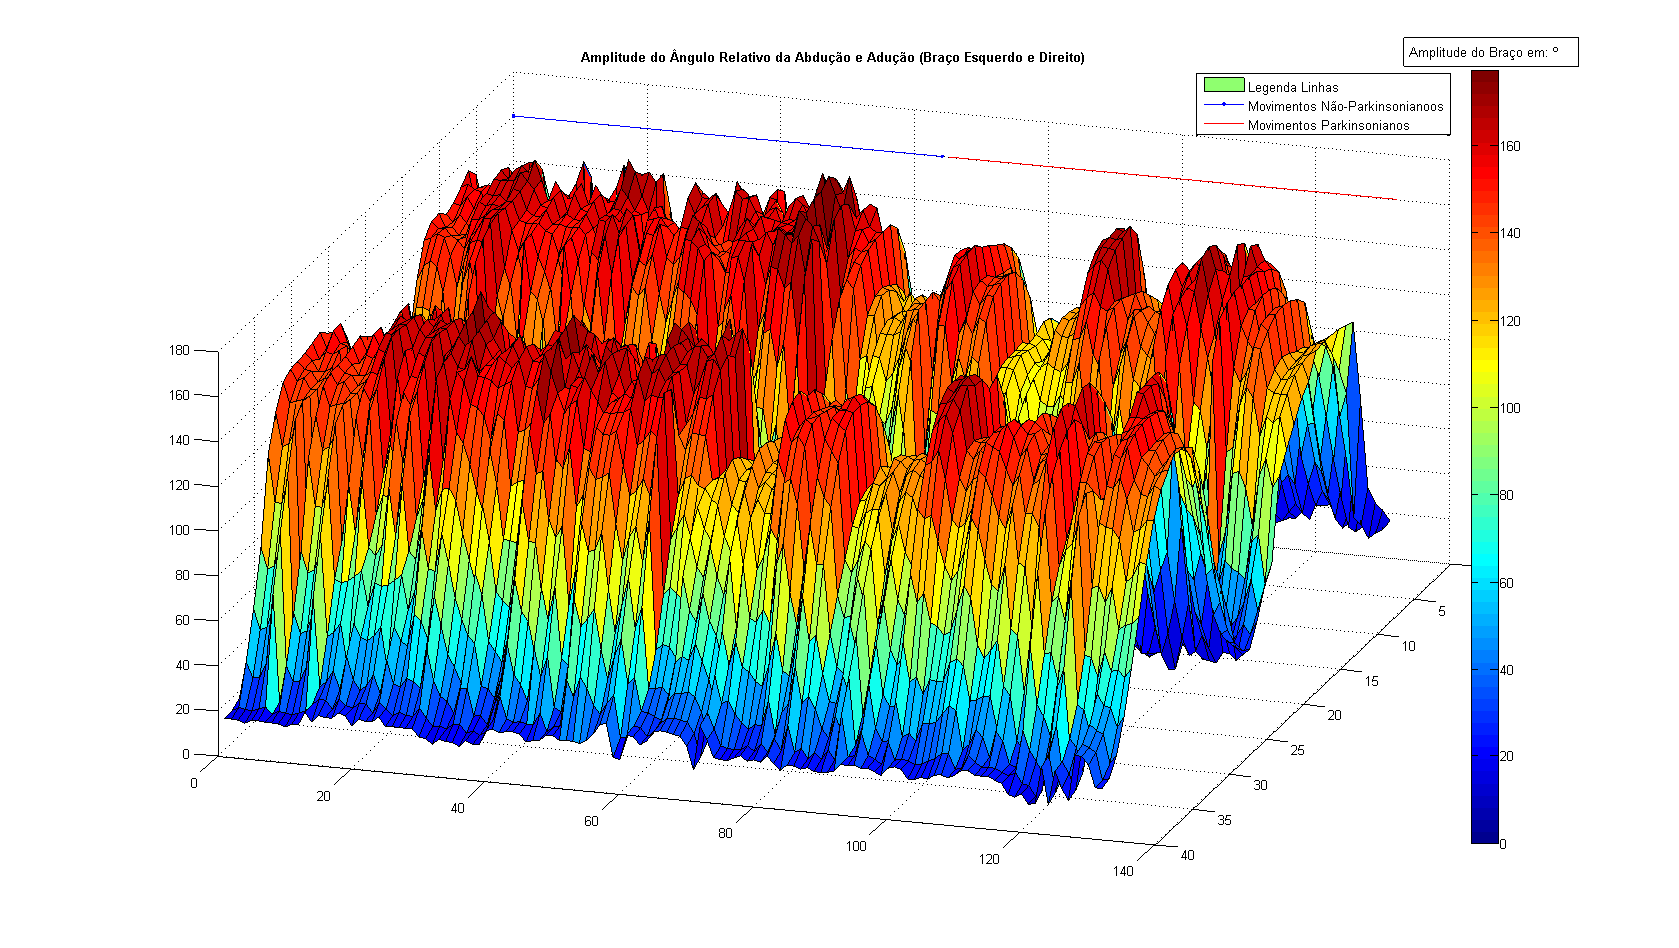
\includegraphics[scale=0.38]{./img/ciclosmovimentokinnect.png}
 \caption{Ciclos de Movimento Abdução e Abdução Usados na Classificação}
 \label{fig:ciclos_movimento_processados_filtrados}
\end{figure}


O vetor de características é composto dos ciclos de movimento e das características extraídas de cada ciclo conforme explicado na Seção~\ref{sec:extracao_caracteristcas}. Ou seja, terá além do ciclo de movimento, os valores da velocidade angular de abdução e adução do braço esquerdo e direito. De posse desse vetor de características e do rótulo sobre a classe do ciclo de movimento (indivíduo diagnosticado com a ~\ac{dp} e indivíduo sem o diagnóstico estabelecido) esses dados serão repassados juntamente como entrada-saída para o classificador de dados que irá dividir entre grupos de treinamento e teste para realizar sua classificação.

Utiliza-se então o classificador de dados como um identificador de possíveis usuários com problemas motores. Logo, o classificador irá auxiliar o profissional de saúde no acompanhamento de seus pacientes. Pois, supondo um profissional de saúde o qual possui um grande número de pacientes que são usuários da abordagem \textit{GAHME} para monitorar seus dados. Um classificador de dados por máquina de aprendizagem seria utilizado para identificar sintomas motores nos indivíduos. Caso um indivíduo fosse identificado com um sintoma pelo classificador, o profissional de saúde poderia visualizar os dados quantificados para realizar a sua tomada de decisão. Logo a responsabilidade da tomada de decisão é do profissional, por esse motivo é que a abordagem \textit{GAHME} serve como apoio ao diagnóstico e acompanhamento dos sintomas motores.


\section{Visualização dos Dados}
O acompanhamento de sintomas motores se faz necessário, principalmente para doenças crônicas de impacto motor e que tenham melhoria nos sintomas. Pois desta forma, auxilia-se o médico no acompanhamento motor e consequentemente permite tratar o paciente de acordo com a resposta ao tratamento.

Como exemplo da abordagem , o profissional de saúde poderia visualizar as características do movimento que serviram como dados de entrada para a máquina de aprendizagem. Nesse caso, podemos ver duas tabelas em que é possível identificar as diferenças motoras de uma pessoa diagnostica com a ~\ac{dp} (Tabela \label{table:extracao_caracterisca_parkinsoniano}) e um indivíduo sem o diagnóstico da doença (Tabela ~\ref{table:extracao-caracteristica}).

\begin{table}[h]
\begin{tabular}{|r|r|r|r|r|r|}
\hline
\multicolumn{4}{|l}{Velocidades º/S}                                                                                                                                                                                                                                                                                         & \multicolumn{2}{|l|}{Amplitudes}     \\ \hline
\multicolumn{1}{|l}{\textbf{\begin{tabular}[c]{@{}c@{}}Abdução\\ Esquerda\end{tabular}}} & \multicolumn{1}{|l|}{\textbf{\begin{tabular}[c]{@{}c@{}}Abdução\\ Direita\end{tabular}}} & \textbf{\begin{tabular}[c]{@{}c@{}}Adução\\ Esquerda\end{tabular}} & \textbf{\begin{tabular}[c]{@{}c@{}}Adução\\ Direita\end{tabular}} & \textbf{Esquerda} & \textbf{Direita} \\ \hline
78,95                                                                                    & 77,82                                                                                    & 83,06                                                              & 106,42                                                            & 130,00            & 124,72           \\ \hline
79,94                                                                                    & 34,68                                                                                    & 104,69                                                             & 39,98                                                             & 131,50            & 132,44           \\ \hline
81,05                                                                                    & 47,05                                                                                    & 107.38                                                             & 56,52                                                             & 132,22            & 123,66           \\ \hline
74,73                                                                                    & 47,09                                                                                    & 109,05                                                             & 47,75                                                             & 132,33            & 122,20           \\ \hline
72,01                                                                                    & 56,02                                                                                    & 102,36                                                             & 76,00                                                             & 131,40            & 119.75      \\ \hline
\end{tabular}
\caption{Extração das Características de Indivíduo Com Diagnóstico da ~\ac{dp}}
\label{table:extracao-caracteristica}
\end{table}

\begin{table}[h]
\begin{tabular}{|r|r|r|r|r|r|}
\hline
\multicolumn{4}{|l}{Velocidades º/S}                                                                                                                                                                                                                                                                                         & \multicolumn{2}{|l|}{Amplitudes}       \\ \hline
\multicolumn{1}{|l}{\textbf{\begin{tabular}[c]{@{}c@{}}Abdução\\ Esquerda\end{tabular}}} & \multicolumn{1}{|l|}{\textbf{\begin{tabular}[c]{@{}c@{}}Abdução\\ Direita\end{tabular}}} & \textbf{\begin{tabular}[c]{@{}c@{}}Adução\\ Esquerda\end{tabular}} & \textbf{\begin{tabular}[c]{@{}c@{}}Adução\\ Direita\end{tabular}} & \textbf{Esquerda} & \textbf{Amplitude} \\ \hline
129,35                                                                                   & 61,59                                                                                    & 78,74                                                              & 176,30                                                            & 159,39            & 143,50             \\ \hline
115,67                                                                                   & 118,15                                                                                   & 71,72                                                              & 79.46                                                             & 156,37            & 153,97             \\ \hline
120.96                                                                                   & 135,27                                                                                   & 66,70                                                              & 78,17                                                             & 154,30            & 149,91             \\ \hline
125.96                                                                                   & 137,43                                                                                   & 64,75                                                              & 81,57                                                             & 153,18            & 154,58             \\ \hline
139.99                                                                                   & 117,60                                                                                   & 69,96                                                              & 84,08                                                             & 151,68            & 148,90             \\ \hline
120,51                                                                                   & 111,92                                                                                   & 75,85                                                              & 75,18                                                             & 152,58            & 148,35             \\ \hline
\end{tabular}
\caption{Extração das Características de Indivíduo Sem Diagnóstico da ~\ac{dp}}
\label{table:extracao_caracterisca_saudavel}
\end{table}

Como pode ser visto nesses dados a amplitude de de um indivíduo diagnosticado com a~\ac{dp} esta bem menor do que um indivíduo sem o diagnóstico estabelecido. Um valor importante também pode ser identificado na velocidade de adução esquerda do indivíduo com ~\ac{dp} possui uma velocidade muito maior do que o indivíduo sem o diagnóstico. Possivelmente porque um paciente da ~\ac{dp} perde um pouco o controle sobre o membro fazendo-o descer abruptamente ~\cite{protpar010}. Desta maneira pretende-se com a abordagem, auxiliar o profissional de saúde com o fornecimento dessa informação para que este venha efetuar o acompanhamento e perceba a evolução do quadro clínico do paciente.

%O produto escalar é uma operação entre dois vetores cujo resultado é um escalar e pode ser descrito na forma:
%$ u.v = |u| |v| cos(\theta) $\ onde $ \theta $\ é o ângulo formado entre $ u $\ e $ v $\ dentro do intervalo de $0 \leq \theta \leq 180º $\.

%Se
%\begin{math}
%v.w = \left \| v \right \|\left \| w \right \|\cos \theta
%\end{math}
%, onde $ \theta $\ é o ângulo entre esses vetores. Então o \textbf{ângulo} entre dois vetores é definido como o menor ângulo entre eles.
%
%Portanto, o ângulo dentro do intervalo de $0 \leq \theta \leq 180º $\ será o resultado do produto interno
%\newline
%\begin{math} \cos \theta = (v.w)/(\left \| v \right \| \left \| w \right \|)\end{math} .

%\subsubsection{Pontos Utilizados no \textit{Ms-Kinnect} Para o Cálculo do Produto Escalar}
%A descrição da posição de um segmento ou movimento articular é tipicamente expressa com relação a uma posição inicial designada. A posição anatômica é uma referência padronizada usada por muitos anos por anatomistas, biomecânicos e médicos ~\cite{hamill1999bases}.



%\begin{figure}
 %\centering
 %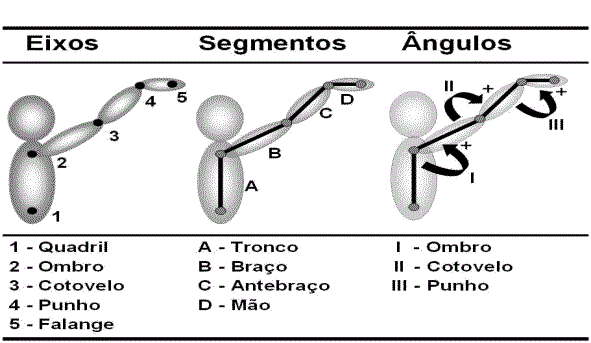
\includegraphics[scale=0.5]{./img/eixossegmentos.png}
 %% matrixargseg.png: 296x162 pixel, 100dpi, 7.52x4.11 cm, bb=0 0 213 117
 %%\caption{Estágio desenvolvimento de jogos ~\cite{fullerton2008game}}
%\caption{Eixos Segmentos e Ângulos da Biomecânica}
%%  \caption{Estágio desenvolvimento de jogos}
 %\label{fig:eixossegmentos}
%\end{figure}
